\chapter{Formales}
\label{chap:Formales}

\section{Erklärung selbständiger Bearbeitung}
Entsprechend der jeweils gültigen Prüfungsordnung ist die vorweggestellte ehrenwörtliche Erklärung notwendiger Bestandteil Ihrer Arbeit. Für Abschlussarbeiten ist Sie zwingend erforderlich.
\section{Formatierung}

% Grundsätzlich gelten folgende Formatvorgaben für die Formatierung:
% 	Gliederung: Max. 3 Hierarchiestufen
% 	Format: DIN A4
% 	Seitenränder: 
% 	links 2,5 cm; 
% 	rechts 2 cm, 
% 	oben 2,5 cm, 
% 	unten 2 cm.
% 	Kopf- und Fußzeile: 
% 	oben 1,5 cm, 
% 	unten 1 cm
% 	Schriftart: Arial oder Calibri (Word 2007)
% 	Schriftgröße:	
% 	11 Punkt im Fließtext
% 	10 Punkt: Abbildungs-, Tabellenbeschriftung und weiter
% 	Zeilenabstand: 1 ½ Zeilen
% 	Absatzformatierung: Blocksatz, mit Silbentrennung
% 	Seitennummerierung: Oben rechts
% 	Beschriftung der Seiten: Einseitig
Sämtliche Vorgaben zur Formatiernug sind in der hier verwendeten Formatvorlage berücksichtigt, so dass Sie diese sofort verwenden können. Bitte nehmen Sie keine Ändungen an den Seitenrändern, Kopf- und Fußzeilen oder der Schriftart vor.

\subsection{Abbildungen und Tabellen}
Tabellen und Abbildungen sind getrennt voneinander und fortlaufend zu nummerieren und immer einheitlich mit einem Titel sowie ggf. der Quelle zu versehen. Es bietet sich an, die Nummerierung an die Kapitelnummer zu koppeln, um eine bessere Übersicht zu gewährleisten. Diese Vorlage berücksichtigt dies und bezieht die Nummer des jeweiligen Kapitels in die Nummerierung von Abbildungen und Tabellen ein. Abbildungen erhalten eine Unterschrift, Tabellen eine Überschrift. Im Text ist mindestens einmal auf jede Abbildungsnummer zu verweisen, gleiches gilt für Tabellen. 
Ein Beispiel für die Tabellenbeschriftung finden Sie in Tabelle \ref{tab:Tabelle}, ein Beispiel für eine Abbildung in \ref{fig:BeispielGraph}.

\begin{table}
	%		\centering
	\caption{Eine Tabellen-Caption}
	%		\rowcolors{2}{white}{gray!15}
	\renewcommand{\arraystretch}{1.3}
	\begin{tabular}{llll}
		\toprule[1pt]
		%			
		& \textsc{Lolimot}	& \textsc{Hilomot} 	& \textsc{Suhiclust}	\\ 
		%								
		\cmidrule[1pt](lr){2-2} \cmidrule[1pt](lr){3-3} \cmidrule[1pt](lr){4-4} %\rowcolor{gray!15} %\midrule[1pt]
		%			
		Teilungsfunktion    & linear 			& linear			& nicht linear \\ 
		Orientierung        & Orthogonal 		& Achsenschräg 		& Achsenschräg \\ %\rowcolor{gray!15}
		Gültigkeitsfunktion	& Sigmoid-Funktion 	& Sigmoid-Funktion 	& Gauß-Funktion \\
		%			
		\bottomrule[1pt]
		\label{tab:Tabelle}
	\end{tabular}
\end{table}

			
			

\subsection{Formelsatz}
Der Formelsatz wird zentriert ausgerichtet. Die Gleichungen sind absatzweise fortlaufend durchzunummerieren. Die Variablen werden kursiv dargestellt, Indizes gerade, sofern sie keine Variable sind. Feststehende Funktionsnamen wie z.B. sin, log sowie Einheiten werden ebenfalls gerade dargestellt, zwischen Zahlenwert und Einheit ist ein Leerzeichen einzufügen. Beispiel: 

\begin{equation}
	e^{i\pi} + 1 = 0
\end{equation}

\subsection{Listings}
Sollten Sie innerhalb des Fließtextes Bezüge beispielsweise zu Elementen benötigten, können Sie dies entweder in Form eines sogenannten Listings, wie in Listing 3.1 dargestellt, oder durch Herausheben des Listing im Text tun. Das Herausheben von Elementen innerhalb des Fließtextes lässt sich mit Hilfe des \verb|\verb|-Befehls erreichen.

Umfassende Listings bspw. für Algorithmen können am besten mit dem Listings-Package erstellt werden. Dieses Package wurde auch für \ref{"listing:SparqlBeispiel} genutzt.

Es kann sinnvoll sein, Elemente aus Listings vorab in den „Typografischen Hinweisen“ festzulegen, insbesondere wenn Sie umfassendere Listings nutzen oder Listings mit Inhalten aus verschiedenen Modellierungs- bzw. Programmiersprachen.

\begin{lstlisting}[mathescape=true, breaklines, language=SPARQL, caption=SPARQL SELECT-WHERE, label="listing:SparqlBeispiel]
PREFIX i: <http://...#>
SELECT * WHERE { 
	?someIndividual rdf:type i:ExampleClass. 
}
\end{lstlisting}

\subsection{Graphen und Kurven}
Die Graphen und Kurven werden in Schriftgröße 11, die Achsen in der Form „x in m“ oder „x/m“ beschriftet. Dabei ist auf eine selbsterklärende Form und deutliche Erklärung durch ausreichende Beschriftung der Graphen und Kurven zu achten. Beispiel: 

\begin{figure}
	\caption{Ein beispielhafter Graph}
	\label{fig:BeispielGraph}
	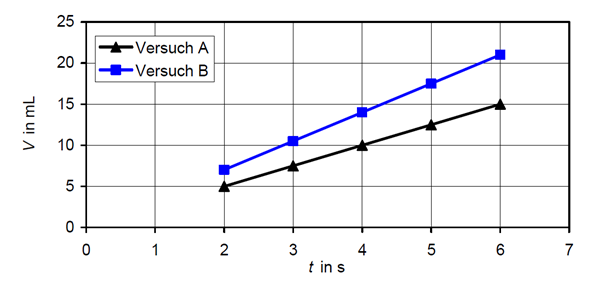
\includegraphics[width=0.9\textwidth]{Inhalt/Abbildungen/Beispiel-Abbildung.png}
\end{figure}

\section{Literaturverzeichnis}
Im Literaturverzeichnis sind alle benutzten Quellen in alphabetischer Reihenfolge der Autoren aufzuführen (Monographien, Sammelveröffentlichungen, usw.). Die einzelnen Quellen werden durch eine Leerzeile voneinander getrennt. Publikationen, die zwar verwendet, d.h. gelesen, in der Arbeit aber nicht erwähnt wurden, gehören nicht ins Literaturverzeichnis. Die Quellen sind wie folgt zu zitieren:
[Kurzbeleg]	Autoren, Titel. Erscheinungsort: Verlag, Erscheinungsjahr.
[Str 98] Strohmann, G.: Automatisierungstechnik 1. Bd. 1. Grundlagen, analoge und digitale Prozessleitsysteme. 4. Auflage München, Wien: Oldenburg, 1998.
\paragraph{Zeitschriften} 
Verfasser: Titel. Bandangabe oder Schriftenreihe. Auflage. Erscheinungsort: Verlag, Erscheinungsjahr. Seitenanzahl des Artikels.
[Fay 05] Fay, A.: Engineering in vernetzten, offenen, durchgängigen Systemen. atp, Heft 4, 05/2005, S. 205-210.
\paragraph{Normen}
Jede Norm ist durch ihre Normierungsgesellschaft und eine von dieser vergebenen Normnummer eindeutig gekennzeichnet. Diese wird zur Kennzeichnung auch in dem Literaturverzeichnis bzw. beim Zitieren verwendet.
DIN 1421 (Ausgabe: Januar 1983): Gliederung und Benennung in Texten: Abschnitte, Absätze, Aufzählungen
\paragraph{Webseiten und Dokumente aus dem Internet} 
Es sind nur Beiträge mit wissenschaftlichem Inhalt zu zitieren. Im Zitat wird zusätzlich zu Angaben über Titel und Autor die Internet-Adresse (URL), die veröffentlichende Organisation (möglichst mit Ort), das Erstellungsdatum und das Abrufdatum angegeben.
Lässt sich keine Person als Autor feststellen, ist der Name der Firma oder der Website zu verwenden. Hat das Dokument keinen Titel, ist es ohne Titel („o.T.“) zu zitieren. Die URL muss auf ein konkretes Dokument verweisen (z.B. \url{http://www.hsu-hh.de/aut/forschung/forschungsthemencrest-modellbasierte-entwicklung-kollaborativer-eingebetteter-systeme}). URLs, die nicht auf konkrete Inhalte verweisen (z.B. http://www.hsu-hh.de) sind nicht zulässig. Als Veröffentlichungsdatum ist die letzte Aktualisierung des Dokuments oder das Speicherdatum anzugeben. 

Angaben im Literaturverzeichnis sind nach folgendem Schema aufzubauen: 

[Krü 05] Krüger, K.: Prozessdatenverarbeitung – Vorlesung. URL: \url{http://www.hsu-hh.de/download1.3.1.htm}. Helmut-Schmidt-Universität (Universität der Bundeswehr Hamburg), 20.07.2005, Abruf am 22.09.2005.
